\documentclass{IEEE}

\begin{document}
\Title{Machine Learning From Disaster}{Calculating the Survival Rate for Passengers in the Titanic}
{Miguel Melo Ochoa}{Alex Hayet}{Francisco Gomez}{Maeki Kashana}
{CS549 - Machine Learning}
{Professor Xin Zhang}
{San Diego State University}


\section{Introduction and Research Problem}
All details for this project will be provided by a competition titled "Titanic - Machine Learning from Disaster" introduced by kaggle.com \cite{titanic}.

This following section will provide a brief background and a statement of the problem this project is addressing.




\subsection{Introduction}

This project will build a predictive model that aims to find the type of people who are going to survive the sinking of the Titanic, a well renowned ship that was believed to be "unsinkable" until it hit an iceberg in 1912, resulting in the death of 1502 passengers/crew.

This project will utilize passenger information, such as name, age, gender, socio-economic class, etc., to determine what sorts of groups were more likely to survive than others during the sinking of the Titanic.

This data aforementioned above will be provided by the Kaggle competition and the goal of this project is to engineer code that uses the data to calculate the survival rate of various groups of people.

\subsection{Research Problem}

This project will be creating a predictive model that will dictate the type of individuals that were the most likely to survive the sinking of the Titanic.

To give more detail, this project will be provided with a lot of testing data in order to make predictions on who will survive. In consequence of this data, this team will be able to create a predictive machine learning model that utilizes the data provided for this project to make predictions using various models previously covered in this course. The specific details regarding any related work that relates to this project will be discussed in depth in later sections.

To get more into specifics, this project will utilize these following .csv files to find a solution for this problem: test.csv and train.csv.


For the train.csv file, it will contain information on who survived the sinking of the Titanic in order to train the model that was developed.

For the test.csv file, it is used to see how well the model that was developed performs on unseen data. This file will be used to make predictions on who survived based on the model that was trained using train.csv.




\section{Related Work}

To create a solution for this project, our code needed to apply the concepts that were learned about logistic regression. To aid with this endeavor, our team utlized the problems that involved logistic regression in Assignment 1.

In this assignment, there was a task that involved training a logistic regression model that classifies two categories of sign language images. Furthermore, through this assignment, we used the forward and backward computation implementation as a reference on implementing a logistic regression model in our own code.

More specifically, our team utilized the equations present in these computations in Assignment 1 and applied them in our code to produce a solution to the Titanic problem. In the forward pass, our team utilized these equations for the activation and the cost: $A=\sigma (w^TX+b)$ and $Cost=-\frac{1}{m}\sum^m_i y^{(i)}log(a^{(i)})+(1-y^{(i)})log(1-a^{(i)})$. In addition, for the backward pass computations, our team utilized these following equations from Assignment 1:
\LIST{
\item $dZ=A-Y$
\item $dw=\frac{1}{m}XdZ^T$

}


\section{Methodology and Technical Details}

\subsection{Methodology}

\subsection{Technical Details}
In regards to the technical details of our code, the two possible outcomes are the person surviving or perishing which are represented as 1 and 0. The independent variables we ended up utilizing were Pclass, Sex, Age, SibSp, Parch, and Embarked. Some of these variables, such as sex, are given as strings so they were changed to binary to make it more convenient to use. This is determined by whether the given passenger’s Sex is male or female and whether their Embarked is Q or S. A few areas also contain nan or “not a number” that had to be replaced with the average value of that category to maintain the patterns found and avoid errors. Once those columns of the Titanic’s passenger data are filtered and modified, it is used to train the model to recognize certain patterns on what increases someone’s chances of survival. That will allow it to make accurate predictions on whether a passenger will survive.

\section{Experimental Results and Analysis}

\subsection{Experimental Results}
Our experimental results for this project are shown in the graphs below. These graphs depict the survivors of the titanic according to our logistic regression model and also these graphs show how the accuracy of the model continues to drop the more iterations there are in the algorithm.

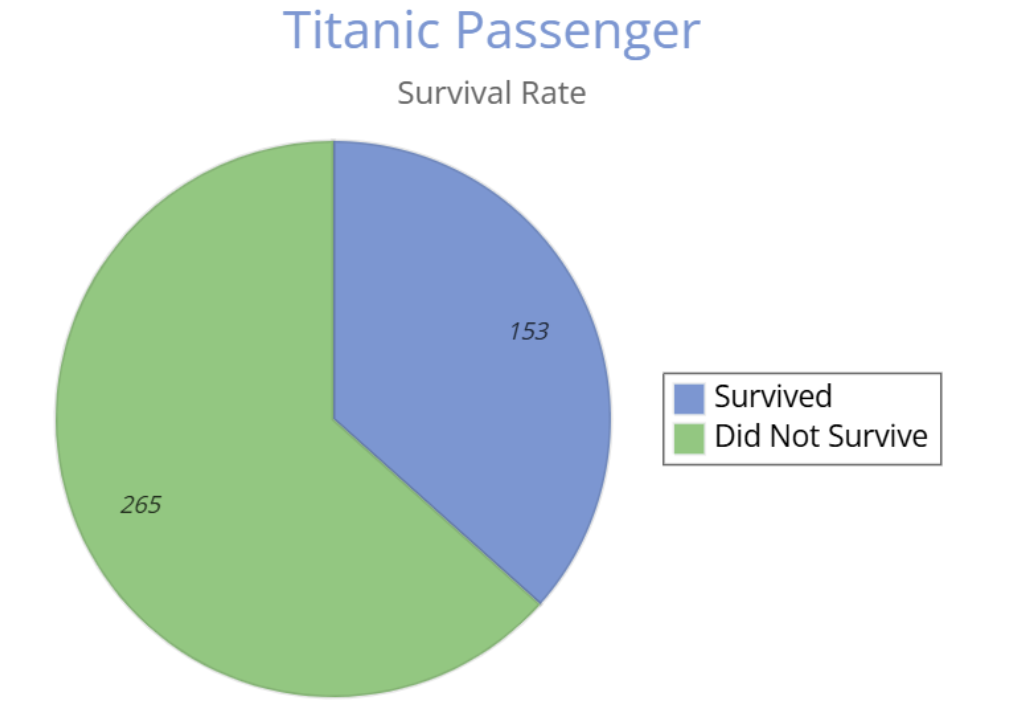
\includegraphics[scale=0.4]{./piechart.png}
\\ 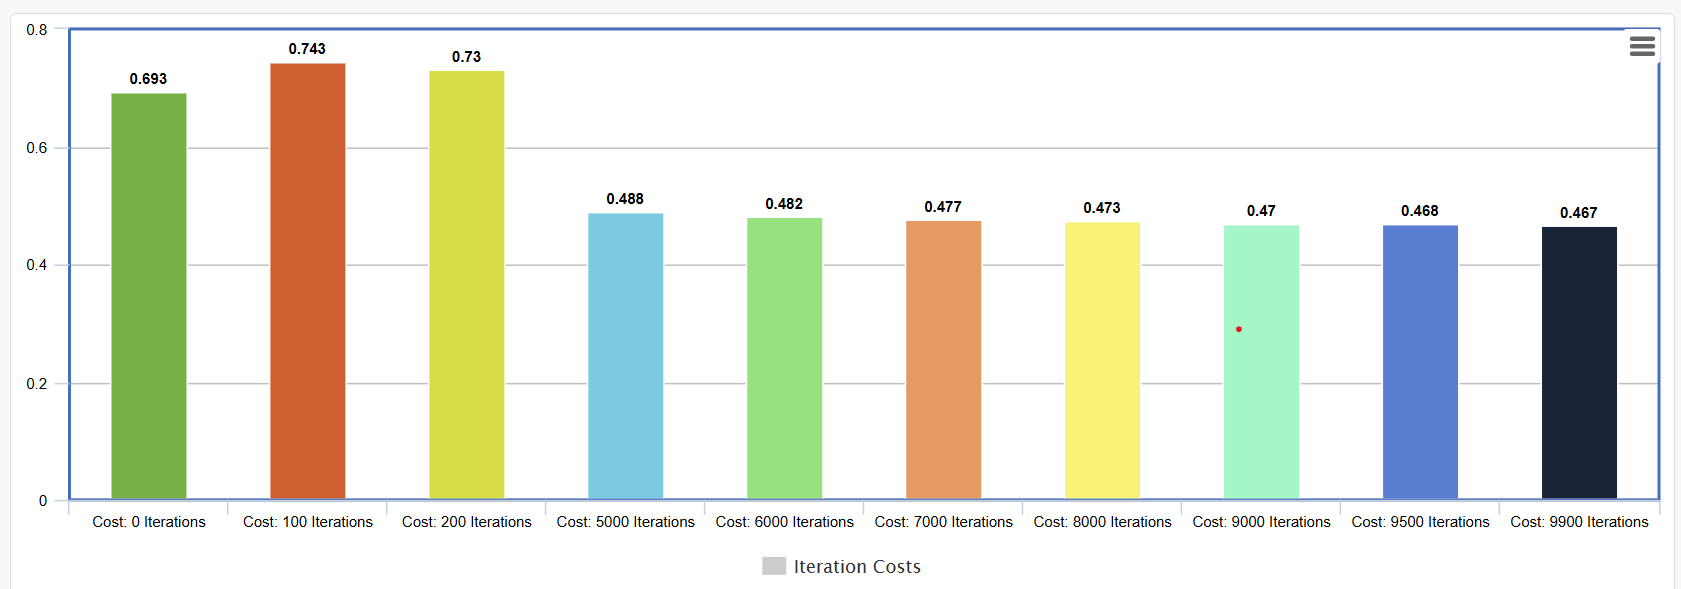
\includegraphics[scale=0.4]{./barchart.png}
\subsection{Analysis}



\section{Conclusion and Future Work}

\subsection{Conclusion}

\subsection{Future Work}





\section{Contributions}

\subsection{Maeki Kashana}
\LIST{
\item Significant Contributions to the Final Report
    \LIST { \item Introduced the Research Problem
            \item Discussed, at length, any past work in the course that relates to this project
            \item Summarized findings and suggested possible future directions}
\item Created the README file
}
\subsection{Miguel Melo Ochoa}
\LIST{
\item
}
\subsection{Alex Hayet}
\LIST{
\item
}
\subsection{Francisco Gomez}
\LIST{
\item Methodology and Technical Details
\item Provided ideas on how to implement the code
}

\REF {
\bibitem{titanic} Cubierski. W., ``Titanic - Machine Learning From Disaster,'' Kaggle.com, 2012.
}
\end{document}
